% !TeX spellcheck = es_ES
\chapter{Experimental}
\label{ch:chap05}

En este capítulo se muestran detalles de las pruebas realizadas, con el objetivo de determinar las características positivas y negativas de los algoritmos implementados en las dimensiones de rendimiento computacional y precisión de los resultados.

\section{Ambiente de prueba}
\label{sec:hardware}

A continuación, se presentan tanto el hardware utilizado en las pruebas (Tabla \ref{table:hardware}) así como las versiones del software utilizado (Tabla \ref{table:software}), de forma que los resultados puedan entenderse en términos relativos al entorno de ejecución utilizado.

\begin{table}[htbp!]
	\centering
	\begin{tabular}{l|l}
		Procesador & Intel i7 8700K - 12 CPUs - 3.7 GHz       \\
		\hline
		GPU        & Nvidia GeForce GTX 1070 Ti - 8 GiB  VRAM \\
		\hline
		RAM        & 32 GiB - 2667 MHz                        \\
		\hline
	\end{tabular}
	\caption{Características del hardware utilizado}
	\label{table:hardware}
\end{table}

\begin{table}[htbp!]
	\centering
	\begin{tabular}{l|l}
	SO & Windows 10 Pro        \\
		\hline
	Embree        & v3.5.2 \\
		\hline
		OpenGL        & v4.5  \\
		\hline
	\end{tabular}
	\caption{Características del entorno de desarrollo utilizado}
		\label{table:software}
\end{table}

\section{Escenas}
\label{sec:escenas}

Con el objetivo de obtener resultados comparables para los distintos algoritmos y configuraciones se plantea el uso de dos escenas particulares de prueba, con distintas variaciones en los materiales que componen cada una de ellas.


\begin{figure}[htbp]
	\centering
	\begin{subfigure}{0.45\textwidth}
		\includegraphics[width=1\linewidth]{assets/cornell}
		\caption{Lateral}
	\end{subfigure}
	\begin{subfigure}{0.45\textwidth}
		\includegraphics[width=1\linewidth]{assets/cornell2}
		\caption{Frontal}
	\end{subfigure}
	\caption{Vistas de la escena \textit{Conrnell Box}.}
	\label{img:cornell}
\end{figure}

Se denomina \textit{Escena - Cornell Box} a la mostrada en la Figura \ref{img:cornell}. Se basa en un tipo de escena comúnmente usado en el que se ubican objetos en el interior de un cubo, donde debajo están los objetos de prueba y en el nivel superior reside el objeto que emitirá luz. Esta escena cuenta con siete objetos: el cubo, una esfera que oficia de luz, y cinco objetos compuestos por diversas primitivas. En total, existen 12.922 polígonos de las cuales 96 son triángulos y 12.826 son cuadriláteros.

\begin{figure}[htbp]
	\centering
	\begin{subfigure}{0.45\textwidth}
		\includegraphics[width=1\linewidth]{assets/street1}
		\caption{Desde la ventana de una de las edificaciones}
	\end{subfigure}
	\begin{subfigure}{0.45\textwidth}
		\includegraphics[width=1\linewidth]{assets/street2}
		\caption{Desde uno de los extremos de la calle}
	\end{subfigure}
	\begin{subfigure}{0.45\textwidth}
		\includegraphics[width=1\linewidth]{assets/street3}
		\caption{Aérea I}
	\end{subfigure}
	\begin{subfigure}{0.45\textwidth}
		\includegraphics[width=1\linewidth]{assets/street4}
		\caption{Aérea II}
	\end{subfigure}
	\caption{Vistas de la escena \textit{Calle}.}
	\label{img:street}
\end{figure}

Se denomina \textit{Escena - Calle} a la referente a la Figura \ref{img:street}. La escena está constituida por dos objetos, el primero de ellos es una cúpula (hemisferio) subdividida en 2.407 cuadriláteros de igual área, cuyo objetivo es representar el cielo. Por otro lado, el segundo objeto es una representación de una porción de una calle en el barrio de Petit Bayonne, localizado en Bayona, Francia cuyas imágenes se aprecian en la figura \ref{img:streetcomp}. El modelo fue construido por Beniot, Acuña, et al. \cite{Benoit} con el objetivo de estudiar el fenómeno de la transferencia de calor a la escala de calle utilizando el método de elementos finitos. En total, la escena cuenta con 61.795 parches cuadrangulares.


\begin{figure}[htbp]
	\centering
	\begin{subfigure}{0.475\textwidth}
		\includegraphics[width=1\linewidth]{assets/streetreal1}
		\caption{Sur - real}
	\end{subfigure}
	\begin{subfigure}{0.475\textwidth}
		\includegraphics[width=1\linewidth]{assets/streetreal2}
		\caption{Norte - real}
	\end{subfigure}
	\begin{subfigure}{0.475\textwidth}
		\includegraphics[width=1\linewidth]{assets/streetmodel1}
		\caption{Sur - modelada}
	\end{subfigure}
	\begin{subfigure}{0.475\textwidth}
		\includegraphics[width=1\linewidth]{assets/streetmodel2}
		\caption{Norte - modelada}
	\end{subfigure}
	\caption{Comparación entre el fotografías reales del modelo \textit{Calle} y su representación tridimensional.}
	\label{img:streetcomp}
\end{figure}

\section{Casos de prueba}
\label{sec:pruebas}

Se proponen casos de prueba utilizando las escenas descritas en la Sección \ref{sec:escenas}, compuestas por diversos materiales.

\subsection{Métricas consideradas}
\label{metricasestablecidas}
Con el objetivo de medir correctamente las ventajas y desventajas de cada método de cálculo de factores de forma simples y extendidos que se han propuesto, se define un conjunto de métricas para evaluar su optimalidad en distintas dimensiones. Cada dimensión se aplica dependiendo del caso considerado.

\begin{itemize}
	\item Rendimiento
		\begin{itemize}
			\item Tiempo de ejecución: Se registra el tiempo empleado en calcular completamente la matriz de factores de forma.
		\end{itemize}
	\item Matriz de factores de forma: Se compara la matriz de control $\mathbf{F_{C}}$, calculada utilizando la técnica de trazado de rayos con una gran resolución (3.145.728 rayos).
		\begin{itemize}
			\item Error relativo promedio por fila: $Ep_{i} = \sum_{j=1}^{N} \frac{|\mathbf{F_{C}}_{ij} -\mathbf{F}_{ij}|}{N \mathbf{F_{C}}_{ij}}$
			\item Error relativo máximo por fila: $Em_{i} = \max_{j=1}^{N}\frac{|\mathbf{F}_{ij} -\mathbf{Fc}_{ij}|}{\mathbf{F_{C}}_{ij}}$
		\end{itemize}
	\item Vector de radiosidad (dado el vector $B$, y el vector de control $Bc$, calculado a partir de la matriz de factores de forma $\mathbf{F_{C}}$):
	\begin{itemize}
		\item Error relativo promedio de radiosidad: $Ep = \sum_{i=1}^{N} \frac{|B_{i}-B_{Ci}|}{N B_{Ci}}$
		\item Error máximo de radiosidad: $Em = \max_{j=1}^{N}|{B_{j} - Bc_{j}}|{B_{Ci}}$
	\end{itemize}
\item Valuación cualitativa:
	\begin{itemize}
		\item Calidad de resultados: Se evaluarán los resultados esperando que se asemejen a la realidad.
	\end{itemize}
\end{itemize}

Las definiciones fueron concebidas con la idea de que es necesario controlar el error de cada etapa del método. Se debe tener especial consideración con los términos geométricos, pues el resultado obtenido en la matriz de factores de forma incidirá en los cálculos posteriores. Para ello, se consideró una buena opción obtener errores relativos por fila, es decir, por parche. Un error promedio bajo asegura que en la generalidad los resultados sean aceptables, mientras que el error máximo controla la varianza del error percibido con el objetivo de evitar casos excepcionales. De la misma manera se considera el error observado en el resultado final, es decir, en el vector de radiosidad. Estos valores incidirán directamente en la calidad de la imagen, aunque pueden ser afectados por el error de la etapa anterior.

\subsection{Descripción de casos de prueba}

\begin{enumerate}
	\item \textit{Prueba difusa}: Se utilizan materiales estrictamente difusos en ambas escenas, cuyos colores no varían a lo largo de las pruebas realizadas. De esta manera se desactiva cualquier interacción especular. Se escoge un conjunto de parches que ofician de fuente luminosa. En caso de la escena \textit{Calle}, se seleccionan 10 parches de la cúpula hemisférica para emular al sol. Por otro lado, para la escena \textit{Cornell Box} se utiliza la bola central como fuente luminosa.
	\item \textit{Prueba especular}: Se utilizan materiales difusos y especulares en ambas escenas, con una cantidad reducida de estos últimos. En caso de la escena \textit{Cornell Box} se utiliza el plano ubicado en el centro como reflector, mientras que en la escena \textit{Calle} se utiliza una selección de ventanas. Para cada \textit{pipeline} (completo) implementado se computa la radiosidad registrando el tiempo de renderizado según la cantidad de muestras configurada.
	\item \textit{Prueba conjunta}: En la escena \textit{Cornell Box} se computarán dos variantes. En una de ellas se utilizan superficies con materiales exclusivamente difusos y en el segundo caso se añaden espejos, con el objetivo principal de destacar diferencias visuales percibidas al utilizar la extensión implementada.
	\item \textit{Prueba de stress}: Se utiliza gran cantidad de espejos en ambas escenas.
\end{enumerate}

\subsection{Resultados observados}

En esta sección se presentan los resultados observados para los casos de prueba planteados. En particular, los resultados se detallan en función de la cantidad de muestras tomadas en cada hemi-cubo o hemisferio según corresponda. Para realizar una comparación justa, se utiliza la misma cantidad de pixeles totales del hemi-cubo como la cantidad de rayos lanzados en el hemisferio. Por ejemplo, para un hemi-cubo donde la cara frontal tiene dimensiones 32x32 pixeles el total de pixeles es de 32x32x3, totalizando 3072 pixeles. Por lo tanto, su caso equivalente en Embree corresponde a lanzar 3072 rayos.

\subsubsection{Caso de prueba I (Reflexión difusa)}

\begin{table}[htbp]
	\centering
	\begin{tabular}{|c|c|l|l||l|l|}
		\hline
		\multicolumn{2}{|c|}{\multirow{2}{*}{\textbf{Muestras}}} & \multicolumn{4}{c|}{\textbf{Tiempo de ejecución (s)}}                                                                                  \\ \cline{3-6} 
		\multicolumn{2}{|c|}{}                   & \multicolumn{2}{c||}{\textit{Cornell Box}}                 & \multicolumn{2}{c|}{\textit{Calle}}                      \\ \cline{1-6}
		\multicolumn{1}{|c|}{OpenGL} &\multicolumn{1}{c|}{Embree} &
		\multicolumn{1}{c|}{OpenGL-D} & \multicolumn{1}{c||}{Embree-D} & \multicolumn{1}{c|}{OpenGL-D} & \multicolumn{1}{c|}{Embree-D} \\ \hline
		\textbf{32x32x3}                        &
		\textbf{3072}                        & 7                           & \textbf{3}                           & 68                          & 14                          \\ \hline
		\textbf{64x64x3}                        &
		\textbf{49512}                       & \textbf{10}                          & 30                          & \textbf{128}                         & 174                         \\ \hline
		\textbf{128x128x3}                        &
		\textbf{196608}                       & \textbf{31}                          & 116                         & \textbf{248}                         & 665                         \\ \hline
		\textbf{256x256x3}                        &
		\textbf{786432}   & \textbf{251}                         & 446                         & \textbf{1213}                        & 2565                        \\ \hline
		\textbf{1024x1024x3}                        &
		\textbf{3145728}                      & \textbf{992}                         & 1778                        & \textbf{4018}                        & 7511                        \\ \hline
	\end{tabular}
	\caption{Resultados obtenidos para el primer caso de prueba. El número de muestras representa la cantidad de píxeles (en OpenGL) y rayos (en Embree) dibujados.}
	\label{tab:tablecaso1}
\end{table}

En este caso, se observa en la Tabla \ref{tab:tablecaso1} que el método del hemi-cubo tiene un rendimiento considerablemente superior al de la traza de rayos. Cabe destacar que se observó una ocupación promedio de la GPU del 30\% y CPU 90\%. Esto probablemente se deba a la gran cantidad de sincronizaciones necesarias entre el dispositivo y el controlador. El uso de traza de rayos presentó una ocupación de la CPU del 99\%. Se destaca la diferencia observada entre OpenGL y Embree en la Figura \ref{plot:emglc1}.

\begin{figure}
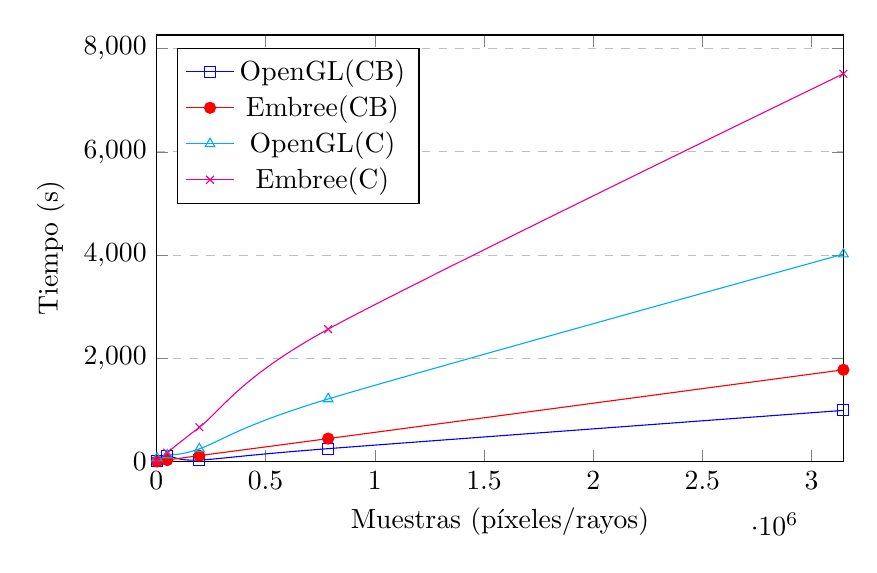
\begin{tikzpicture}
\begin{axis}[
xlabel={Muestras (píxeles/rayos)},
ylabel={Tiempo (s)},
xmin=0, xmax=3145728,
ymin=0,
width=.85\textwidth, height=7cm,
legend pos=north west,
ymajorgrids=true,
grid style=dashed,
]

\addplot[
smooth,
color=blue,
mark=square,
]
coordinates {
	(3072,7)(49512,105)(196608,31)(786432,251)(3145728,992)
};
\addplot[
smooth,
color=red,
mark=*,
]
coordinates {
	(3072,3)(49512,30)(196608,116)(786432,446)(3145728,1778)
};

\addplot[
smooth,
color=cyan,
mark=triangle,
]
coordinates {
	(3072,68)(49512,128)(196608,248)(786432,1213)(3145728,4018)
};

\addplot[
smooth,
color=magenta,
mark=x,
]
coordinates {
	(96,14)(49512,174)(196608,665)(786432,2565)(3145728,7511)
};

\legend{OpenGL(CB),Embree(CB),OpenGL(C), Embree(C)}

\end{axis}
\end{tikzpicture}
\caption{Comparación del rendimiento de los algoritmos en escenas exclusivamente difusas}
\label{plot:emglc1}
\end{figure}

Una de las consecuencias más interesantes a ser analizadas para detectar la cantidad de muestras óptimas a considerar es la calidad de la imagen final, y qué tan pronunciadas son las diferencias en la iluminación entre los parches, es decir, en qué medida difiere la radiosidad entre parches. Para este caso, se pudo observar (véase la Figura \ref{img:difres}) que si bien las resoluciones más bajas consumen menor cantidad de recursos los resultados tienen una calidad sustancialmente menor. Considerando que el modelo generalmente es utilizado para el cálculo de iluminación en una etapa de pre-procesado (fuera de línea), es recomendable evitar el uso de factores de muestreo tan bajos. Esto se ve acentuado en el análisis de la matriz de factores de forma, según las métricas establecidas en \ref{metricasestablecidas} se pudo comprobar que máximo error promedio apreciado (medida que se ha denominado $Ep$) fue de $0,05$ y $0,04$ utilizando $786.432$ muestras para los métodos del hemi-cubo y el hemisferio mientras que el uso de $3.072$ muestras generó errores del entorno de los $0,14$ y $0,06$ respectivamente. Estos se ven aún más acentuados al realizar el cálculo de la radiosidad para cada parche.

\begin{figure}[htbp]
	\centering
	\begin{subfigure}{0.45\textwidth}
		\includegraphics[width=1\linewidth]{assets/32sgl}
		\caption{OpenGL - 32 píxeles por cara}
	\end{subfigure}
	\begin{subfigure}{0.45\textwidth}
		\includegraphics[width=1\linewidth]{assets/512sgl}
		\caption{OpenGL - 512 píxeles por cara}
	\end{subfigure}
	\begin{subfigure}{0.45\textwidth}
		\includegraphics[width=1\linewidth]{assets/32srt}
		\caption{Embree - 3072 rayos}
	\end{subfigure}
	\begin{subfigure}{0.45\textwidth}
		\includegraphics[width=1\linewidth]{assets/512srt}
		\caption{Embree - 786432 rayos}
	\end{subfigure}
	\caption{Diferencias visuales ajustando la cantidad de muestras}
	\label{img:difres}
\end{figure}

\subsubsection{Caso de prueba II (Reflexión Difusa + Especular)}

En este caso, se observa en la tabla \ref{tab:caso2} que el mejor rendimiento se obtiene utilizando el método híbrido, esto se debe a los hilos que ejecutan los cálculos correspondientes al rebote especular (utilizando traza de rayos) son ejecutados en la CPU mientras la GPU procesa hemi-cubos. Esta observación se ve respaldada por el hecho de que, en promedio se observó una ocupación rondando en los entornos de 100\% de la CPU y 35\% GPU en el método híbrido, 75\% de la CPU y 30\% GPU en el método utilizando OpenGL y 99\% en la implementación que solo utiliza traza de rayos. 

\begin{table}[htbp!]
	\centering
	\begin{tabular}{|l|l|l|l|l||l|l|l|}
		\hline
		\multicolumn{2}{|c|}{\multirow{2}{*}{\textbf{Muestras}}} & \multicolumn{6}{c|}{\textbf{Tiempo de ejecución (s)}}                                                                                  \\ \cline{3-8} 
		\multicolumn{2}{|c|}{}                   & \multicolumn{3}{c||}{\textit{Cornell Box}}                 & \multicolumn{3}{c|}{\textit{Calle}}                      \\ \cline{1-8}
		\multicolumn{1}{|c|}{OpenGL} &\multicolumn{1}{c|}{Embree} & \multicolumn{1}{c|}{GL-D+S} & \multicolumn{1}{c|}{E-D+S} & \multicolumn{1}{c||}{Híb} & GL-D+S                 & E-D+S & Híb \\ \hline
		\textbf{32x32x3 - 32}                                &
		\textbf{3072x3 - 32}                                & 25                         & 53                          & \textbf{21}                           & 2563                   & 1221   & \textbf{943}     \\ \hline
		\textbf{256x256x3 - 32}                                &
		\textbf{196608 - 32}                               & 93                         & 134                         & \textbf{84}                          & \textbf{1054}                   & 2512   & 1643    \\ \hline
		\textbf{512x512x3 - 64} &\textbf{786432 - 64}                              & 304                        & 486                         & \textbf{228}                          & \multicolumn{1}{c|}{-} & 5342   & \textbf{4725}    \\ \hline
	\end{tabular}
	\caption{Resultados obtenidos en el segundo caso de prueba. Notación: GL, E, Híb corresponden a OpenGL, Embree e Híbrido. La notación 'D+S' indica que se utilizaron reflexiones difusas y especulares. Los valores de muestras a la derecha indican la resolución de los espejos. '-' indica casos de prueba que tomaron tiempos excesivos.}
	\label{tab:caso2}
\end{table}

El paralelismo de las implementaciones basadas en la GPU garantiza el mejor rendimiento, sin embargo, se pudo notar que el uso exclusivo de traza de rayos provee hasta 800 veces menor error máximo que los otros algoritmos implementados. En \textit{Cornell Box}, con 786.432 muestras se notó una diferencia de error máxima $Ep$ de $0,0080$ con el método híbrido y $0,0055$ utilizando el método de dibujado de portales, en comparación con el método de traza de rayos que logró un error de $0,1 \times 10^{-3}$.

\begin{table}[htbp!]
	\centering
	\begin{tabular}{|l|l|l|l|l|}
		\hline
		\multicolumn{2}{|c|}{\multirow{2}{*}{\textbf{Muestras}}} & \multicolumn{3}{c|}{\textbf{Error relativo (normalizado)}}\\ \cline{3-5} 
		\multicolumn{2}{|c|}{}                   & \multicolumn{3}{c|}{\textit{Cornell Box}}                                \\ \cline{1-5}
		\multicolumn{1}{|c|}{OpenGL} &\multicolumn{1}{c|}{Embree} & \multicolumn{1}{c|}{GL-D+S} & \multicolumn{1}{c|}{E-D+S} & \multicolumn{1}{c|}{Híb} \\ \hline
		\textbf{32x32x3 - 32}                                &
		\textbf{3072 - 32}                                & 0.0138                         & 0.000481                          & 0.0091                                \\ \hline
		\textbf{256x256x3 - 32}                               &
		\textbf{196608 - 32}                               & 0.0093                         & 0.000108                         & 0.0073                             \\ \hline
		\textbf{512x512x3 - 64} &\textbf{786432 - 64}                              & 0.0080                        & 0.000010                         & 0.0055                             \\ \hline
	\end{tabular}
	\caption{Resultados obtenidos en el segundo caso de prueba (Cornell Box).}
	\label{tab:caso2err}
\end{table}

Esto se debe a que tanto en el uso de dibujado de portales o el algoritmo híbrido se utilizan estimaciones de la dirección en la que rebotaría el rayo en el espejo considerado, lo que degrada la autenticidad final de los datos obtenidos, sobre todo en el dibujado de portales donde la granularidad de las muestras obtenidas es inferior (se toman muestras por área y no por rayo). Por lo tanto, incluso si el método de traza de rayos posee un tiempo de ejecución un tanto mayor (que se debe mayormente al hecho de que se ejecuta únicamente en la CPU) se observa una calidad de datos de órdenes de magnitud superior a la de los otros métodos.

\begin{figure}[htpb!]
	\centering
	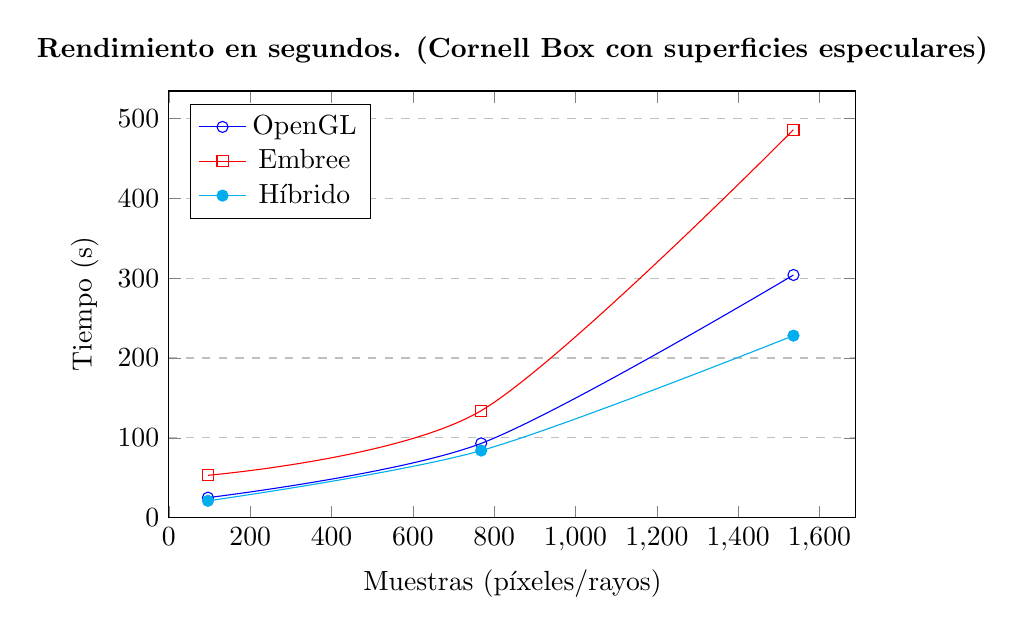
\begin{tikzpicture}
	\label{plot:emglc2}
	\begin{axis}[
	title={\textbf{Rendimiento en segundos. (Cornell Box con superficies especulares)}},
	xlabel={Muestras (píxeles/rayos)},
	ylabel={Tiempo (s)},
	xmin=0,
	ymin=0,
	width=.85\textwidth, height=7cm,
	legend pos=north west,
	ymajorgrids=true,
	grid style=dashed,
	]
	
	\addplot[
	smooth,
	color=blue,
	mark=o,
	]
	coordinates {
		(96,25)(768,93)(1536,304)
	};
	\addplot[
	smooth,
	color=red,
	mark=square,
	]
	coordinates {
		(96,53)(768,134)(1536,486)
	};
	
	\addplot[
	smooth,
	color=cyan,
	mark=*,
	]
	coordinates {
		(96,21)(768,84)(1536,228)
	};
	
	
	\legend{OpenGL,Embree,Híbrido}
	
	\end{axis}
	\end{tikzpicture}
	\caption{Rendimiento en segundos, considerando superficies especulares}
\end{figure}


\begin{figure}[htbp!]
	\centering
	\begin{subfigure}{0.5\textwidth}
		\includegraphics[width=1\linewidth]{assets/cornellesp2}
		\caption{OpenGL-D+S}
	\end{subfigure}
	\begin{subfigure}{0.5\textwidth}
		\includegraphics[width=1\linewidth]{assets/cornellespembree}
		\caption{Embree-D+S}
	\end{subfigure}
	\begin{subfigure}{0.5\textwidth}
		\includegraphics[width=1\linewidth]{assets/caso3esp}
		\caption{Híbrido}
	\end{subfigure}	
	\caption{Diferencias visualizadas utilizando las distintas implementaciones de cálculo de factores de forma extendido. 1536 muestras iniciales y 64 para rebotes especulares.}
	\label{img:difres2}
\end{figure}

Con el objetivo de cuantificar los datos de error observado se analizó el error promedio en el vector de radiosidad final (comparado a una muestra utilizando exclusivamente trazado de rayos con 786.432 muestras para el hemisferio) y se constató que, tal como se había supuesto, el método es significativamente menos propenso a generar errores como se ve en la Figura \ref{img:difres2}.

\begin{figure}[htbp!]
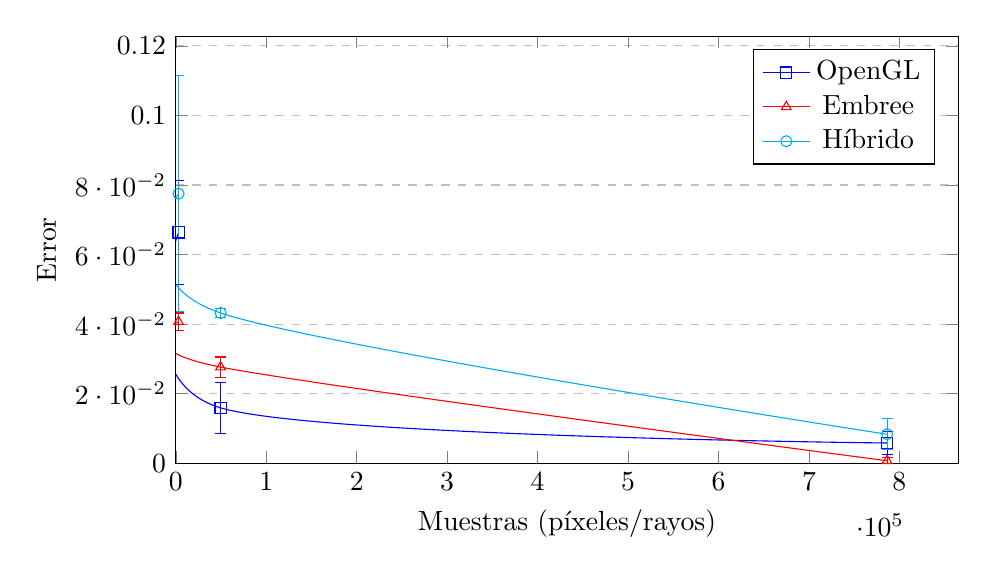
\begin{tikzpicture}
\begin{axis}[
xlabel={Muestras (píxeles/rayos)},
ylabel={Error},
xmin=0,
ymin=0,
width=.95\textwidth, height=7cm,
legend pos=north east,
ymajorgrids=true,
grid style=dashed,
]

\addplot[
smooth,
color=blue,
mark=square,
mark=square,error bars/.cd, y dir=both,y explicit
]
coordinates {
	(3072,0.06634) +- (0, 0.015)
	(49512,0.01593) +- (0, 0.0074)
	(786432,0.00582) +- (0, 0.0034)
};
\addplot[
smooth,
color=red,
mark=triangle,
mark=triangle,error bars/.cd, y dir=both,y explicit
]
coordinates {
	(3072,0.0406985) +- (0, 0.0025)
	(49512,0.02765) +- (0, 0.0029)
	(786432,0.000712) +- (0, 0.0009)
};

\addplot[
smooth,
color=cyan,
mark=* ,
mark=o,error bars/.cd, y dir=both,y explicit
]
coordinates {
	(3072,0.0775)  +- (0, 0.034)
	(49512,0.0432)  +- (0, 0.0014)
	(786432,0.008324)  +- (0, 0.0045)
};


\legend{OpenGL,Embree,Híbrido}

\end{axis}
\end{tikzpicture}
\caption{Error promedio observado en valor final de radiosidad en Híbrido. Los intervalos muestran el error máximo.}
\label{plot:errorcII}
\end{figure}

\subsubsection{Caso de prueba III (Conjunta)}

Esta prueba se construyó con el objetivo de comparar el rendimiento observado utilizando los algoritmos para el cálculo de factores de forma extendidos implementados. Es interesante comparar las diferencias en los tiempos de ejecución para una cantidad de muestras fijas, incluso si se han notado grandes discrepancias entre los resultados observados entre los métodos. Se ha puesto especial énfasis en las diferencias producidas al variar la cantidad de caras especulares de la escena, es decir, los parches cuyo coeficiente de reflexión es positivo. Las pruebas se realizaron con una cantidad de muestras fijas (256x256x3 para el hemi-cubo o 196.608 rayos para Embree y 4.096 muestras para el portal).

\begin{table}[htbp!]
	\centering
	\caption{Pruebas realizadas en \textit{Cornell Box} para identificar incidencia en la cantidad de caras especulares utilizadas en el tiempo de ejecución}
\begin{tabular}{|l|l|l|l|}
	\hline
	\multicolumn{1}{|c|}{\textbf{Parches especulares}} & \multicolumn{1}{c|}{OpenGL (s)} & \multicolumn{1}{c|}{Embree (s)} & \multicolumn{1}{c|}{Híbrido (s)} \\ \hline
	\textbf{0}                              & \textbf{38}                          & 126                         & -                            \\ \hline
	\textbf{16}                             & 41                          & 118                         & \textbf{39}                           \\ \hline
	\textbf{32}                             & 48                          & 120                         & \textbf{40}                           \\ \hline
	\textbf{64}                             & 68                          & 121                         & \textbf{43}                           \\ \hline
\end{tabular}
	\label{tab:caso3}
\end{table}

En la Tabla \ref{tab:caso3} puede observarse cómo la traza de rayos supera en dos veces el tiempo a los otros algoritmos. Sin embargo, se ha de destacar (al igual que en las pruebas anteriores) que los resultados observados tendrían variaciones en caso de utilizarse resoluciones mayores para el dibujado de portales. En cuyo caso, los tiempos entre los casos de prueba serían más afines, aunque se conseguirían resultados peores dada las aproximaciones realizadas en el dibujado de portales. Esto se demuestra al emparejar la cantidad de muestras tomadas por el portal con las de cada cara del hemi-cubo (256); en este caso los tiempos de ejecución para $62$ parches especulares es de 150 segundos. Por lo tanto, si bien existe un tiempo de ejecución mayor la estabilidad (en tiempo de ejecución) y la calidad de los datos obtenidos hacen que el método de traza de rayos sea superior a las otras dos propuestas.

\begin{figure}[htbp!]
	\centering
	\begin{subfigure}{0.47\textwidth}
		\includegraphics[width=1\linewidth]{assets/streete}
		\caption{Extensión desactivada}
	\end{subfigure}
	\begin{subfigure}{0.47\textwidth}
		\includegraphics[width=1\linewidth]{assets/streets}
		\caption{Extensión activada}
	\end{subfigure}
	\caption{Diferencias observadas activando y desactivando extensiones}
	\label{img:difspecstreet}
\end{figure}

Adicionalmente, como se puede observar en la Figura \ref{img:difspecstreet}, las diferencias obtenidas en el valor final de la iluminación en cada parche pueden ser sutiles no obstante asemejan la simulación a escenarios reales con un costo despreciable en el tiempo de ejecución. En esta prueba en particular, se notó un aumento de aproximadamente 20 segundos (de 670 a 690). Donde en el primer caso se utilizó únicamente la iluminación difusa mientras que en segundo caso se activó la extensión utilizando trazado de rayos.

\subsubsection{Caso de prueba IV (Stress)}

Finalmente, con el objetivo de evaluar el impacto de contar con muchas superficies especulares se probó qué tanto tiempo adicional insume la carga impuesta al algoritmo del hemisferio (Embree) para considerar este tipo de superficie. Los resultados pueden observarse en la Figura \ref{plot:este}. Se notó una diferencia máxima de 3\% del tiempo de cálculo de los factores de forma al variar la cantidad de superficies especulares entre 0 y 1500 parches. Es por ello que se puede concluir que al utilizar algoritmos de traza de rayos no se detecta un impacto significativo en el tiempo de ejecución.

\begin{figure}[htbp!]
	\centering
	\resizebox{0.7\textwidth}{!}{
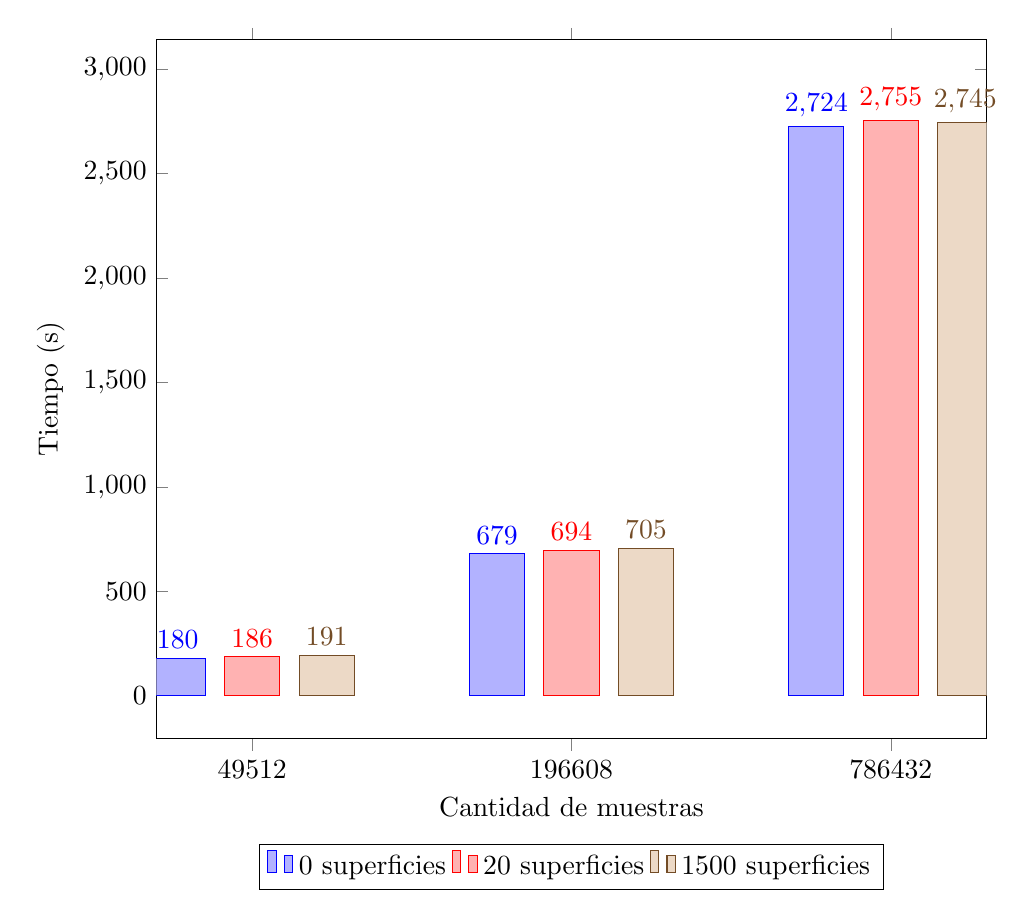
\begin{tikzpicture}

\begin{axis}[
ybar=7pt,
enlargelimits=0.15,
bar width=0.7cm,
legend style={at={(0.5,-0.15)},
	anchor=north,legend columns=-1},
ylabel={Tiempo (s)},
xlabel={Cantidad de muestras},
symbolic x coords={49512,196608,786432},
xtick=data,
nodes near coords,
nodes near coords align={vertical},
width=\linewidth
]
\addplot coordinates {(49512,180) (196608,679) (786432,2724)};
\addplot coordinates {(49512,186) (196608,694) (786432,2755)};
\addplot coordinates {(49512,191) (196608,705) (786432,2745)};
\legend{0 superficies, 20 superficies, 1500 superficies}
\end{axis}
\end{tikzpicture}}
\caption{Variación en el tiempo de ejecución en función de la cantidad de muestras y superficies especulares}
\label{plot:este}
\end{figure}

